\documentclass[border=2pt]{standalone}
\usepackage{tikz}
\usetikzlibrary{positioning,arrows.meta,shapes.geometric,fit,calc}
\usepackage{amsmath,amssymb}
\begin{document}
    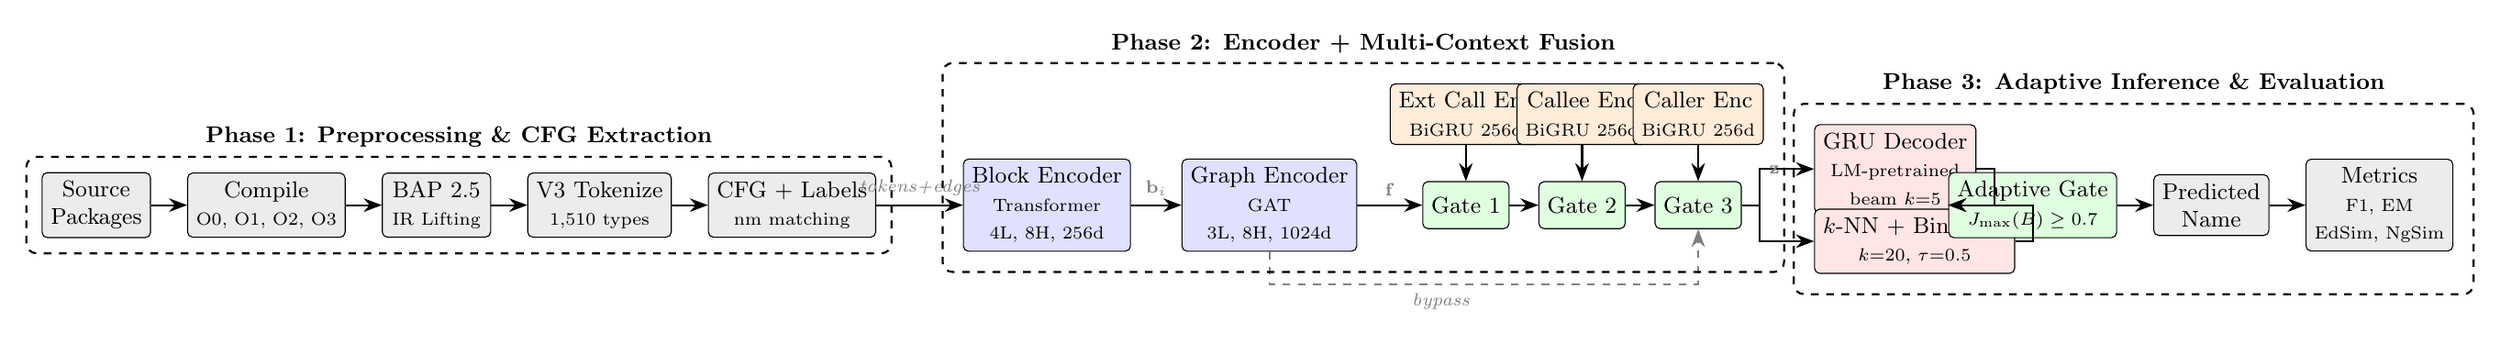
\begin{tikzpicture}[
        node distance=0.4cm and 0.5cm,
        box/.style={rectangle, draw, rounded corners=2pt, minimum height=0.65cm, minimum width=1.5cm, align=center, font=\small},
        phase/.style={rectangle, draw, rounded corners=4pt, thick, dashed, inner sep=6pt},
        stage/.style={box, fill=blue!12},
        context/.style={box, fill=orange!15},
        gate/.style={box, fill=green!12, minimum width=1.1cm},
        output/.style={box, fill=red!10},
        input/.style={box, fill=gray!15},
        arr/.style={-{Stealth[length=2.5mm]}, thick},
        bypass/.style={-{Stealth[length=2.5mm]}, thick, dashed, gray},
        lbl/.style={font=\scriptsize\itshape, text=gray},
    ]
    % === Phase 1: Preprocessing ===
    \node[input] (src) {Source\\Packages};
    \node[input, right=of src] (compile) {Compile\\{\scriptsize O0, O1, O2, O3}};
    \node[input, right=of compile] (bap) {BAP 2.5\\{\scriptsize IR Lifting}};
    \node[input, right=of bap] (tokens) {V3 Tokenize\\{\scriptsize 1,510 types}};
    \node[input, right=of tokens] (cfg) {CFG + Labels\\{\scriptsize nm matching}};

    \draw[arr] (src) -- (compile);
    \draw[arr] (compile) -- (bap);
    \draw[arr] (bap) -- (tokens);
    \draw[arr] (tokens) -- (cfg);

    \node[phase, fit=(src)(compile)(bap)(tokens)(cfg), label={[font=\small\bfseries]above:Phase 1: Preprocessing \& CFG Extraction}] (p1) {};

    % === Phase 2: Model ===
    \node[stage, right=1.2cm of cfg] (blockenc) {Block Encoder\\{\scriptsize Transformer}\\{\scriptsize 4L, 8H, 256d}};
    \node[stage, right=0.7cm of blockenc] (gat) {Graph Encoder\\{\scriptsize GAT}\\{\scriptsize 3L, 8H, 1024d}};

    \draw[arr] (cfg) -- node[above, lbl] {tokens\\+edges} (blockenc);
    \draw[arr] (blockenc) -- node[above, lbl] {$\mathbf{b}_i$} (gat);

    % Fusion
    \node[gate, right=0.9cm of gat] (fuse1) {Gate 1};
    \node[gate, right=0.4cm of fuse1] (fuse2) {Gate 2};
    \node[gate, right=0.4cm of fuse2] (fuse3) {Gate 3};

    \node[context, above=0.5cm of fuse1] (ext) {Ext Call Enc\\{\scriptsize BiGRU 256d}};
    \node[context, above=0.5cm of fuse2] (callee) {Callee Enc\\{\scriptsize BiGRU 256d}};
    \node[context, above=0.5cm of fuse3] (caller) {Caller Enc\\{\scriptsize BiGRU 256d}};

    \draw[arr] (gat) -- node[above, lbl] {$\mathbf{f}$} (fuse1);
    \draw[arr] (fuse1) -- (fuse2);
    \draw[arr] (fuse2) -- (fuse3);
    \draw[arr] (ext) -- (fuse1);
    \draw[arr] (callee) -- (fuse2);
    \draw[arr] (caller) -- (fuse3);

    % Bypass
    \draw[bypass] (gat.south) -- ++(0,-0.45) -| node[below, pos=0.2, lbl] {bypass} (fuse3.south);

    \node[phase, fit=(blockenc)(gat)(fuse1)(fuse2)(fuse3)(ext)(callee)(caller), inner sep=8pt, label={[font=\small\bfseries]above:Phase 2: Encoder + Multi-Context Fusion}] (p2) {};

    % === Phase 3: Inference & Evaluation ===
    \node[output, right=1.0cm of fuse3, yshift=0.5cm] (decoder) {GRU Decoder\\{\scriptsize LM-pretrained}\\{\scriptsize beam $k{=}5$}};
    \node[output, right=1.0cm of fuse3, yshift=-0.5cm] (knn) {$k$-NN + BinFilter\\{\scriptsize $k{=}20$, $\tau{=}0.5$}};
    \node[gate, right=0.6cm of $(decoder)!0.5!(knn)$] (agate) {Adaptive Gate\\{\scriptsize $J_{\max}(B)\ge 0.7$}};
    \node[input, right=0.5cm of agate] (name) {Predicted\\Name};
    \node[input, right=0.5cm of name] (metrics) {Metrics\\{\scriptsize F1, EM}\\{\scriptsize EdSim, NgSim}};

    \draw[arr] (fuse3.east) -- ++(0.25,0) |- node[above right, lbl, pos=0.3] {$\mathbf{z}$} (decoder.west);
    \draw[arr] (fuse3.east) -- ++(0.25,0) |- (knn.west);
    \draw[arr] (decoder.east) -- ++(0.25,0) |- (agate.west);
    \draw[arr] (knn.east) -- ++(0.25,0) |- (agate.west);
    \draw[arr] (agate) -- (name);
    \draw[arr] (name) -- (metrics);

    \node[phase, fit=(decoder)(knn)(agate)(name)(metrics), inner sep=8pt, label={[font=\small\bfseries]above:Phase 3: Adaptive Inference \& Evaluation}] (p3) {};

    \end{tikzpicture}%

\end{document}
